% !TEX TS-program = pdflatex
% !TEX encoding = UTF-8 Unicode

\documentclass[a4paper, titlepage=false, parskip=full-, 10pt]{scrartcl}

\usepackage[utf8]{inputenc}
\usepackage[T1]{fontenc}
\usepackage[english, ngerman]{babel}
\usepackage{babelbib}
\usepackage{hyperref}
\usepackage{listings}
\usepackage{framed}
\usepackage{color}
\usepackage{graphicx}
\usepackage[normalem]{ulem}
\usepackage{cancel}
\usepackage{amsmath}
\usepackage{amssymb}
\usepackage{amsthm}
\usepackage{algorithm}
\usepackage{algorithmic}
\usepackage{geometry}
\usepackage{subfigure}
\geometry{a4paper, top=20mm, left=35mm, right=25mm, bottom=40mm}

\newcounter{tasknbr}
\setcounter{tasknbr}{1}
\newenvironment{task}[1]{{\bf Aufgabe \arabic {tasknbr}\stepcounter{tasknbr}} (#1):\begin{enumerate}}{\end{enumerate}}
\newcommand{\subtask}[1]{\item[#1)]}

% Listings -----------------------------------------------------------------------------
\definecolor{red}{rgb}{.8,.1,.2}
\definecolor{blue}{rgb}{.2,.3,.7}
\definecolor{lightyellow}{rgb}{1.,1.,.97}
\definecolor{gray}{rgb}{.7,.7,.7}
\definecolor{darkgreen}{rgb}{0,.5,.1}
\definecolor{darkyellow}{rgb}{1.,.7,.3}
\lstloadlanguages{C++,[Objective]C,Java}
\lstset{
escapeinside={§§}{§§},
basicstyle=\ttfamily\footnotesize\mdseries,
columns=fullflexible, % typewriter font look better with fullflex
keywordstyle=\bfseries\color{blue},
% identifierstyle=\bfseries,
commentstyle=\color{darkgreen},      
stringstyle=\color{red},
numbers=left,
numberstyle=\ttfamily\scriptsize\color{gray},
% stepnumber=5,
% numberfirstline=true,
breaklines=true,
% prebreak=\\,
showstringspaces=false,
tabsize=4,
captionpos=b,
% framexrightmargin=-.2\textwidth,
float=htb,
frame=tb,
frameshape={RYR}{y}{y}{RYR},
rulecolor=\color{black},
xleftmargin=15pt,
xrightmargin=4pt,
aboveskip=\bigskipamount,
belowskip=\bigskipamount,
backgroundcolor=\color{lightyellow},
extendedchars=true,
belowcaptionskip=15pt}

%% Enter current values here: %%
\newcommand{\lecture}{Algorithmische Geometrie SS15}
\newcommand{\tutor}{}
\newcommand{\assignmentnbr}{11}
\newcommand{\students}{Julius Auer, Alexa Schlegel}
%%-------------------------------------%%

\begin{document}  
{\small \textsl{\lecture \hfill \tutor}}
\hrule
\begin{center}
\textbf{Übungsblatt \assignmentnbr}\\
[\bigskipamount]
{\small \students}
\end{center}
\hrule

\begin{task}{Konfliktecken}
\item[]
Beschreiben Sie in Einzelheiten die Initialisierung der Konfliktstruktur beim randomisierten inkrementellen Algorithmus zur Berechnung des Schnitts von Halbräumen in $\mathbb{R}^3$.
\end{task}


\begin{task}{randomisiert inkrementelle Kontruktionen}
\item[]
Geben Sie randomisiert inkrementelle Algorithmen an zur Konstruktion folgender Strukturen für endliche Punktmengen im $\mathbb{R}^2$

\subtask{a} konvexe Hülle
Hier könnte eigentlich der Algo hin den wir auch in der VL besprochen haben. Man startet mit 3 Punten und bestimmt einen Punkt im Inneren. Dann zieht man von ihm aus gesehen Strahlen zu den 3 äußeren Punkten und hat somit Kegel. Wenn nun ein neuer Punkt hinzukommt wird der Kegel bestimmt in dem der neue Punkt liegt. Verbinen und immer überprüfen ob es eine links bzw. rechtskurve ist, d.h im bzw. gegen den Urzeigersinn bestehende konvexe Hülle durchsuchen. Falls falsche Kurve dann geht man weiter und nimmt den nächsten Punkt. (TODO schöner aufschreiben)

\subtask{b} Voronoi-Diagramm
Gegeben ist die Punktmenge $P=\{p_1, \dots, p_n\} \in \mathbb{R}^2$. Der folgende randomisierte inkrementelle Algorithmus konstuiert das Voronoi-Diagramm $VD(P)$.

Im $i-$ten Schritt ist $VD(p_1, \dots, p_i)$ gegeben, der Punkt $p_{i+1}$ möchte eingefügt werden:

(1) Bestimme die Voronio Region für den Punkt~$p_{i+1}$, also $VR(p_{i+1})$ (das geht in $O(n)$). Die Region heiß~$r$ und der zugehörige Punkt~$p_r$.\\


(2) Konstruiere orthogonale Gerade zu $\overline{p_{i+1}, p_r}$ \\

(3) Bestimme die Schnittpunkte der Gerade mit allen Voronio Kanten der Region~$r$. Da gibt es 0, 1 oder 2 Stück. Vielleicht kann man die in eine Liste packen.\\

Solange die Liste der Schnittpunkte nicht leer ist:\\


(4) $s$ wird neue Voronoi Ecke\\

(5) durch $s$ getroffene Voronoi Kante wird bestimmt. der eine Punkt davon wird weggeschmissen, die Kante verkürzt\\
(6) rausfinden welche Voronio Region zu der Kante noch gehört, den Punkt davon bestimmen\\
(7) Orthogonale Gerade zwischen diesem Punkt und $p_i+1$ aufstellen und Schnittpunkte mit der Region bestimmen, Schnittpunkt zur Liste hinzufügen und bei (4) weitermachen. Voronio Kante zwischen dem neu gefunden Schnittpunkt und altem einfügen.

Irgendwie kann man die nicht sofort wegschmeißen und kürzen, einfach hinterher machen.

Laufzeit:\\
(1) $O(n)$\\
(2) $O(1)$\\
(3) wie viele Kanten gibts denn?\\
insgesamt $O(n)$\\

(Todo so formulieren, dass man es versteht.)

\begin{figure}[htpb]
\begin{center}
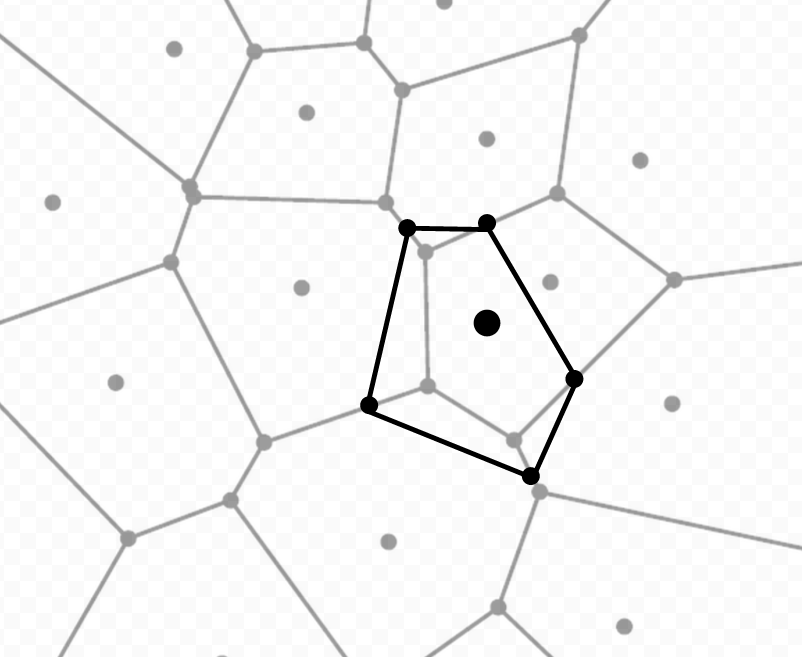
\includegraphics[width=7cm]{vd.png}
\end{center}
\caption{TODO}
\end{figure}


\end{task}

\end{document}